\chapter{Results}
\label{ch:results}

This chapter presents the results of the realizations conducted in the previous chapter. It proposes an analysis of the next steps that someone in the future could take to improve the system.

\section{Objectives fullfilement}
\subsection{Recording system}

Once we installed the recording system on the HEIA-FR building, it allowed us to record the street at any time and generate large amounts of data. The system was reliable, always available, and thanks to the script to run it, it was also easy to use.

\paragraph*{Problems encountered}

We first tried streaming the data directly from the raspberry pi to the storage server with the Real-time Transport Protocol (RTP) \footnote{\url{https://fr.wikipedia.org/wiki/Real-time\_Transport\_Protocol}}. By default, the RTP protocol did not encrypt the streamed data. The \textit{ffmpeg} encoding buffer was regularly full, which caused the loss of some frames and some artifacts in the audio, and the streaming technique gave us a bad image quality due to the real-time encoding of the video.

We solved all these problems by using the SFTP protocol. We solved the image quality by mounting the storage server's folder on the raspberry pi as a network driver. Since ffmpeg no longer used the RTP, it could take his time to encode the video in good quality and save it. The SFTP use also solved the buffer issue. Finally, the SFTP protocol allowed us to encrypt the data since it's a secure protocol by default. An example of the difference between the two method's quality can be seen in the figure \ref{fig:streaming}.

\begin{figure}[H]
    \centering
    \subfloat[Frame quality with RTP]{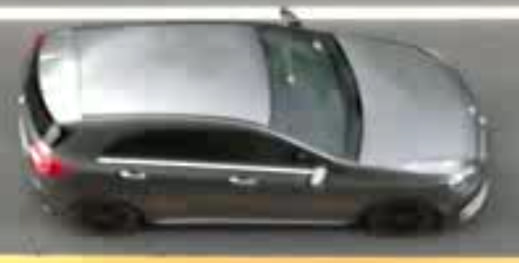
\includegraphics[width=0.45\textwidth]{images/streaming_rtp.png}\label{fig:streaming_rtp}}
    \qquad
    \subfloat[Frame quality with SFTP]{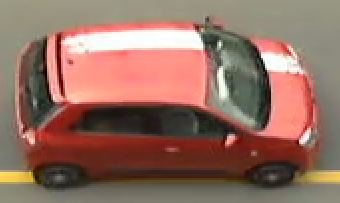
\includegraphics[width=0.45\textwidth]{images/streaming_sftp.png}\label{fig:streaming_sftp}}
    \caption{Comparison of the frame quality between the two streaming methods}
    \label{fig:streaming}
\end{figure}

Even if the quality difference is not considerable, getting a better quality by using the SFTP protocol was a nice side effect of changing the streaming method.

\section{Definition of the baseline}

With the analysis and design parts of the report (section \ref{sec:baseline_analysis} and \ref{sec:baseline_design}), we defined the baseline as a set of steps to follow to achieve the goal of this project. The baseline described in this report is accurate and complete enough to be followed by someone else in the future. The definition achieves the first objective of creating a baseline in section \ref{intro:objective1}. 

\section{Real-life dataset}

With the recording system in place, we built a dataset for this project comprising 2028 dual-channel audio and video files of 2 seconds classified into four classes. The realization of this dataset achieves the goal defined in section \ref{intro:objective2} of having a dataset that follows the baseline to train our model. The dataset is complete and follows the baseline. It is also large enough to train a model with it. The dataset's creation solves the problem of the lack of a dataset for this project. We can consider the objective defined in section \ref{intro:objective2} as achieved.

Although the dataset is created and follows the baseline, it is questioned in the next section ()\ref{sec:neural_network_results}).

\section{Neural Network model results}
\label{sec:neural_network_results}

We trained the neural network multiple times and tested it on the test set. The results were not as good as expected. The model was not able to classify the \textit{no\_car} and the \textit{multiple\_cars} classes very well. The model could not accurately classify the \textit{right\_to\_left} and \textit{left\_to\_right} classes. We trained the model with different percentages of the dataset in the train set. First with 60\%, then with 70\%, and finally with 80\%.
The results are presented in the table \ref{tab:neural_network_results}.

\begin{figure}[H]
    \centering
    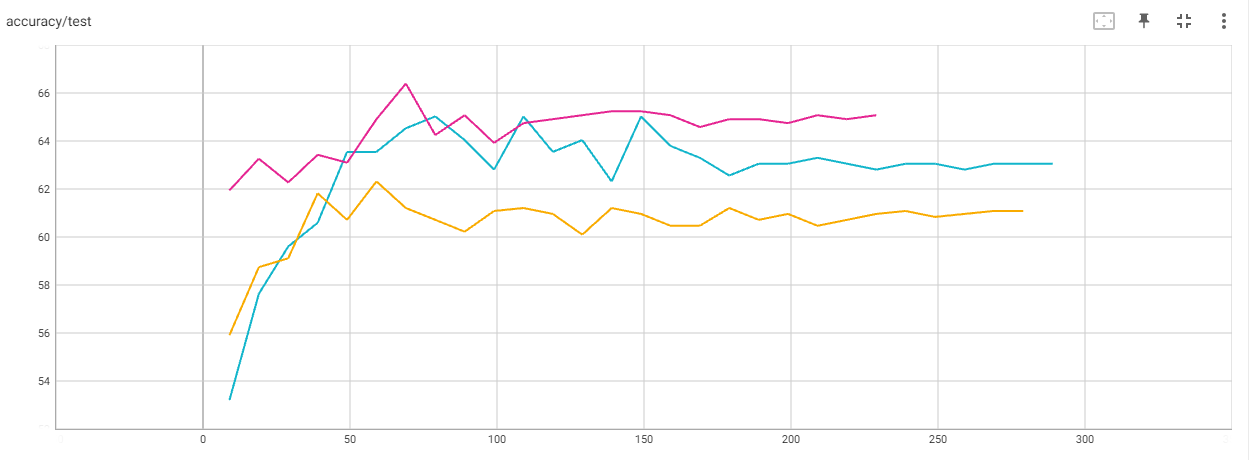
\includegraphics[width=1\textwidth]{images/accuracy_test.png}
    \caption{Accuracy of the neural network model for each train set proportion. Orange is 60\%, purple is 70\%, and pink is 80\%}
    \label{ftab:neural_network_results}
\end{figure}

We can see that the model trained with 70\% of the dataset in the train set is the one that has the best accuracy. It might mean that using the 80\% dataset in the train set is too much, and the model overfits the data. If we look at the loss graph (figure \ref{fig:loss_test}), we can see that the model trained with 60\% of the dataset in the train set has a higher loss than the two others. 

\begin{figure}[H]
    \centering
    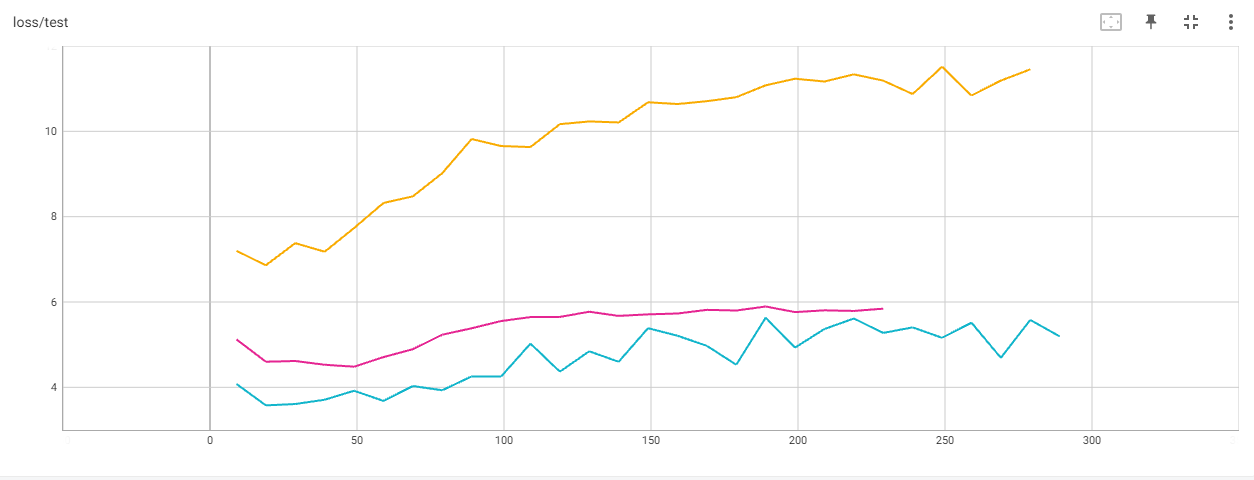
\includegraphics[width=1\textwidth]{images/loss_test.png}
    \caption{Loss of the neural network model each train set proportion. Orange is 60\%, purple is 70\%, and pink is 80\%}
    \label{fig:loss_test}
\end{figure}

The accuracy and loss of the models are presented in the next table. We added the runs with the 40\%, 50\%, and 90\% of the dataset in the train set to the table \ref{tab:neural_network_results} to show that the model's accuracy and loss are not better with these percentages.

\begin{table}[H]
    \centering
    \begin{tabular}{|l|l|l|l|}
    \hline
    \textbf{Train set} & \textbf{Test set} & \textbf{Test set accuracy} & \textbf{Test set loss} \\ \hline
    40\%               & 60\%              & 0.60              & 21.3        \\ \hline
    50\%               & 50\%              & 0.61              & 9.5         \\ \hline
    60\%               & 40\%              & 0.63              & 11.4        \\ \hline
    70\%               & 30\%              & 0.65              & 5,84        \\ \hline
    80\%               & 20\%              & 0.61              & 5.1         \\ \hline
    90\%               & 10\%              & 0.50              & 6.3         \\ \hline
    \end{tabular}
    \caption{Accuracy and loss of the neural network model for each train set percentage}
    \label{tab:neural_network_results}
\end{table}

We can see in the table \ref{tab:neural_network_results} that the model trained with 70\% of the dataset in the train set has the best accuracy and loss. We can also see that the 90\% one has the worst accuracy and loss. We can see that the loss with the small train set is big, so the model cannot generalize well. This observation concludes that we need a bigger dataset to train the model.

To better understand with which classes the model is not performing well, we can look at the confusion matrix of the model trained with 70\% of the dataset in the train set (figure \ref{fig:confusion_matrix}).

\begin{figure}[H]
    \centering
    \subfloat[Epoch 5 (start of the training)]{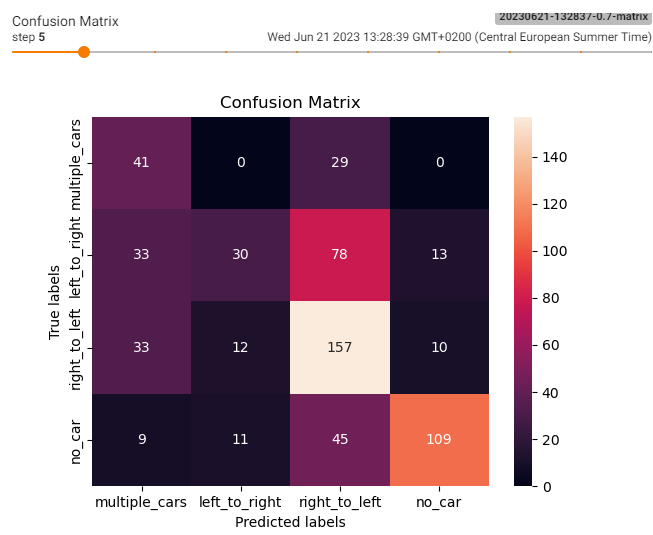
\includegraphics[width=0.7\textwidth]{images/confusion_matrix_epoch_5.png}}
    \qquad
    \subfloat[Epoch 80 (end of the training)]{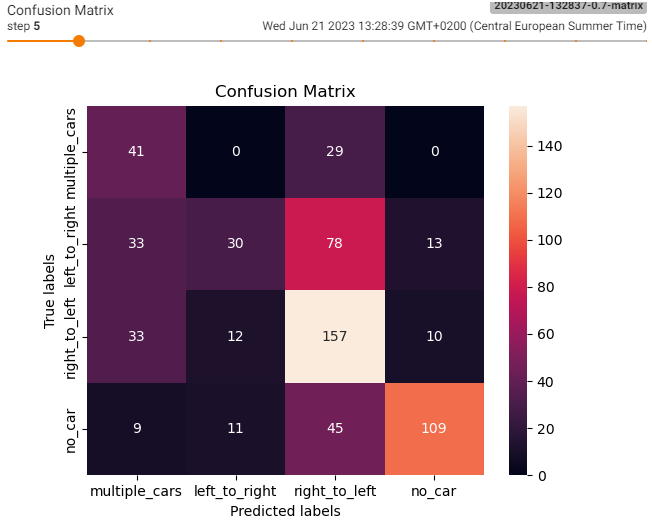
\includegraphics[width=0.7\textwidth]{images/confusion_matrix_epoch_80.png}}
    \caption{Confusion matrix of the model trained with 70\% of the dataset in the train set}
    \label{fig:confusion_matrix}
\end{figure}

We can see that the model can classify well on the first epochs between the \textit{no\_car} and the \textit{multiple\_car} class. We can see it by looking at the four corners of the confusion matrix. The corners on the top-left and bottom-right have a high number, while the ones in the bottom left and the top right have a small number.

On the last epoch, the model better predicts the two classes \textit{left\_to\_right} and \textit{right\_to\_left}. We can see it by looking at the center of the last epoch of the confusion matrix. Overall, we might have a case of overfitting. To solve this problem, we have multiple possibilities.

\begin{itemize}
    \item We can do an early stopping of the training. We can stop the training when the loss on the test set starts to increase. 
    \item We also can construct a bigger dataset. Since we could train the model on more data, it would generalize better and be less likely to overfit.
\end{itemize}

We also have a dataset that is hard to tell when a vehicle is coming from the left or the right. This problem seems to be hard. We could train the model with more data to predict these classes better. We tried to train the model with more parameters to see if it could get better accuracy. We added more convolutional layers and more neurons in the fully connected layers, but the results were not better than this model. To not make the model too big, we decided to keep this model.

\subsection{Human accuracy}

We annotated the test set with only the audio to compare the human and model performance. At this task, the human did only 30.3\% of accuracy. This accuracy is just slightly better than average. We can see on the confusion matrix (figure \ref{fig:human_score_only_audio}) that the human has difficulty telling when there is a vehicle. He predicted more than 50\% of the classes as \textit{no\_car}. 

\begin{figure}[H]
    \centering
    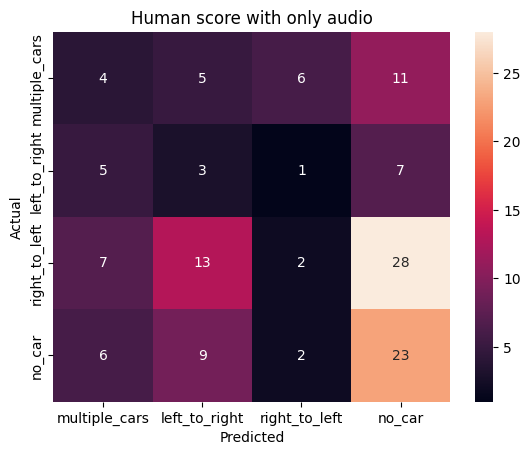
\includegraphics[width=1\textwidth]{images/human_score_only_audio.png}
    \caption{confusion matrix of the human on the audio classified set}
    \label{fig:human_score_only_audio}
\end{figure}

To have a fair comparison, we tested the model on the same dataset that the human was confronted to. The model achieved a score of 63.08\% with the following confusion matrix (figure \ref{fig:model_score_only_audio}):

\begin{figure}[H]
    \centering
    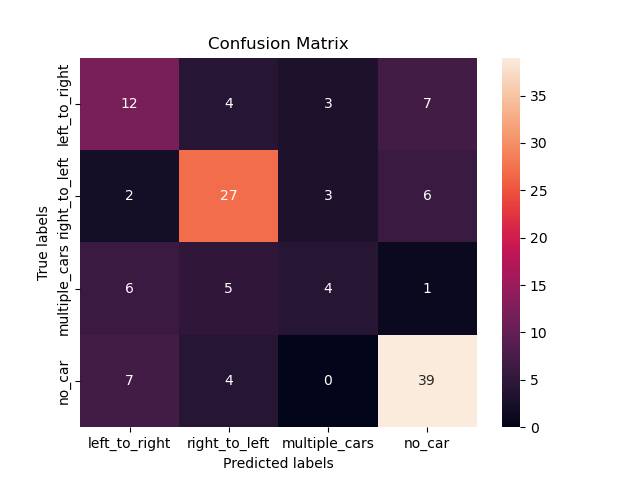
\includegraphics[width=1\textwidth]{images/model_score_only_audio.png}
    \caption{confusion matrix of the model on the test set}
    \label{fig:model_score_only_audio}
\end{figure}

We can see that the model performs way better than the human. 

With this result, we can tell that the objective \ref{intro:objective3} is achieved. The model is better than humans at predicting the vehicle's direction with only the audio input. Still, the model could be way better. Achieving 63.08\% of accuracy is not enough to be used in a real-life situation. With this model, we have a complete baseline definition and can try to improve the score.

\subsection{Dataset quality}

With the results from the convolutional neural network, it's hard to tell if the dataset is well labeled or not. We can see that the model can classify the \textit{no\_car} and the \textit{multiple\_cars} classes very well. The model could not accurately classify the \textit{right\_to\_left} and \textit{left\_to\_right} classes. This could mean that the dataset is not well labeled.

\subsection{Dataset Augmentation with the Simulation}
\label{sec:augmentation_results}

By adding the simulated data to the real-life dataset, we hoped to see better accuracy for the model. We will call it the augmented dataset. The augmented dataset keeps the same number of real-life samples in the train and test sets. We augment the train with the simulation data. We can see in the table \ref{tab:neural_network__augmented_results} that the model trained with 70\% of the dataset in the train set has the best accuracy and loss. We can also see that the 90\% one has the worst accuracy and loss. We can see that the loss with the small train set is big, so the model cannot generalize well. This observation concludes that we need a bigger dataset to train the model.

\begin{table}[H]
    \centering
    \begin{tabular}{|l|l|l|}
    \hline
    \textbf{Train set} & \textbf{Real-Life} & \textbf{Augmented} \\ \hline
    40\%               & 61.71              & 59.06         \\ \hline
    50\%               & 61.2               & 61.22         \\ \hline
    60\%               & 61.08              & 61.62         \\ \hline
    70\%               & 63.77              & 64.1          \\ \hline
    80\%               & 63.05              & 60.64         \\ \hline
    90\%               & 59.5               & 59.31         \\ \hline
    \end{tabular}
    \caption{Accuracy comparisons between the real-life and the augmented dataset for each train set percentage}
    \label{tab:neural_network__augmented_results}
\end{table}

We can see in the table \ref{tab:neural_network__augmented_results} that the augmented dataset does not improve the model's accuracy. We can see that the model trained with 70\% of the dataset in the train set has the best accuracy and loss. We can also compare the confusion matrix of both models (figure \ref{fig:confusion_matrix}). We can see that the augmented dataset does not change a lot the confusion matrix.

\begin{figure}[H]
    \centering
    \subfloat[Real-life dataset]{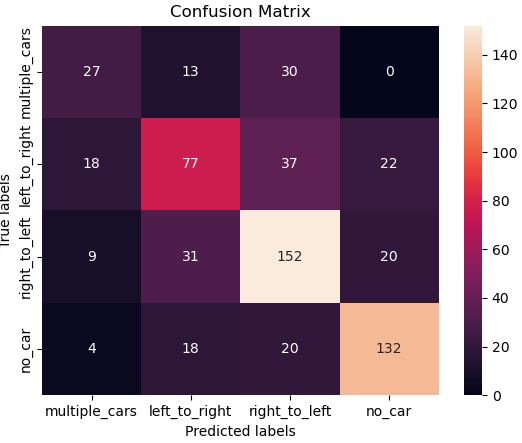
\includegraphics[width=0.7\textwidth]{images/confusion_matrix_real_life.png}\label{fig:confusion_matrix_real_life}}
    \qquad
    \subfloat[Augmented dataset]{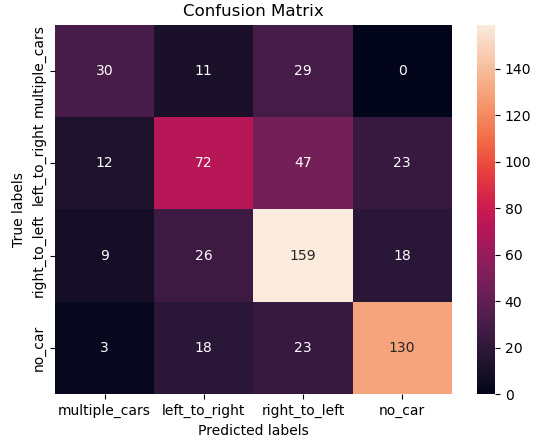
\includegraphics[width=0.7\textwidth]{images/confusion_matrix_augmented.png}\label{fig:confusion_matrix_augmented}}
    \caption{Confusion matrix of the model trained with 70\% of the dataset in the train set}
    \label{fig:confusion_matrix}
\end{figure}

We can deduce that the simulated data does not help the model. The reason might be that the simulated data is unrealistic, so the models ignore it. It might happen because there are errors in the simulation, and the generated data contains them.

The objective \ref{intro:objective4} was to augment the dataset with the simulation. We only partially fulfilled this objective. We have created a dataset in a simulation, but it does not help the model.

\section{Adversarial Attack results}

The adversarial attacks were realized on the best model of the convolutional neural network. We use the model that uses 70\% of the dataset (Table \ref{tab:neural_network_results}).

We took every input from the test set that is classified correctly by the convolutional neural network. We try the FGSM with the following $epsilons$: 1e-08, 1e-07, 1e-06, 1e-05, 0.0001, 0.001, 0.01, 0.1, 1.0, 10.0. For each epsilon, we modify the input we chose previously and use it to predict again on the model. This attack gives us the following graph (Figure \ref{fig:fgsm_results}).

\begin{figure}[H]
    \centering
    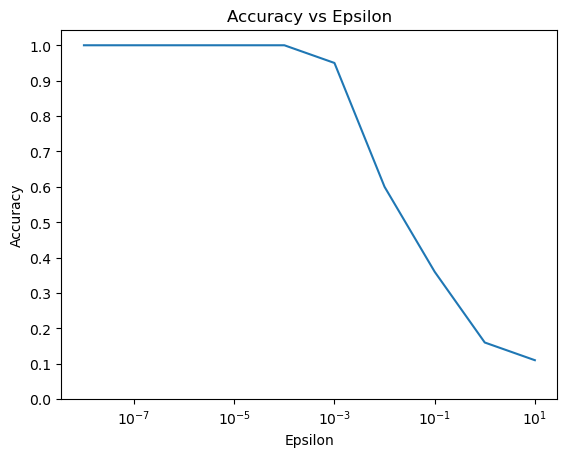
\includegraphics[width=0.8\textwidth]{images/fgsm_results.png}
    \caption{Accuracy of the model for each epsilon value with the FGSM attack}
    \label{fig:fgsm_results}
\end{figure}

We can see that the accuracy is dropping around $10^-3$ and $10^-1$. We can visualize what happens to the input with the following images (Figure \ref{fig:adversarial_attack_results}).

\begin{figure}[H]
    \centering
    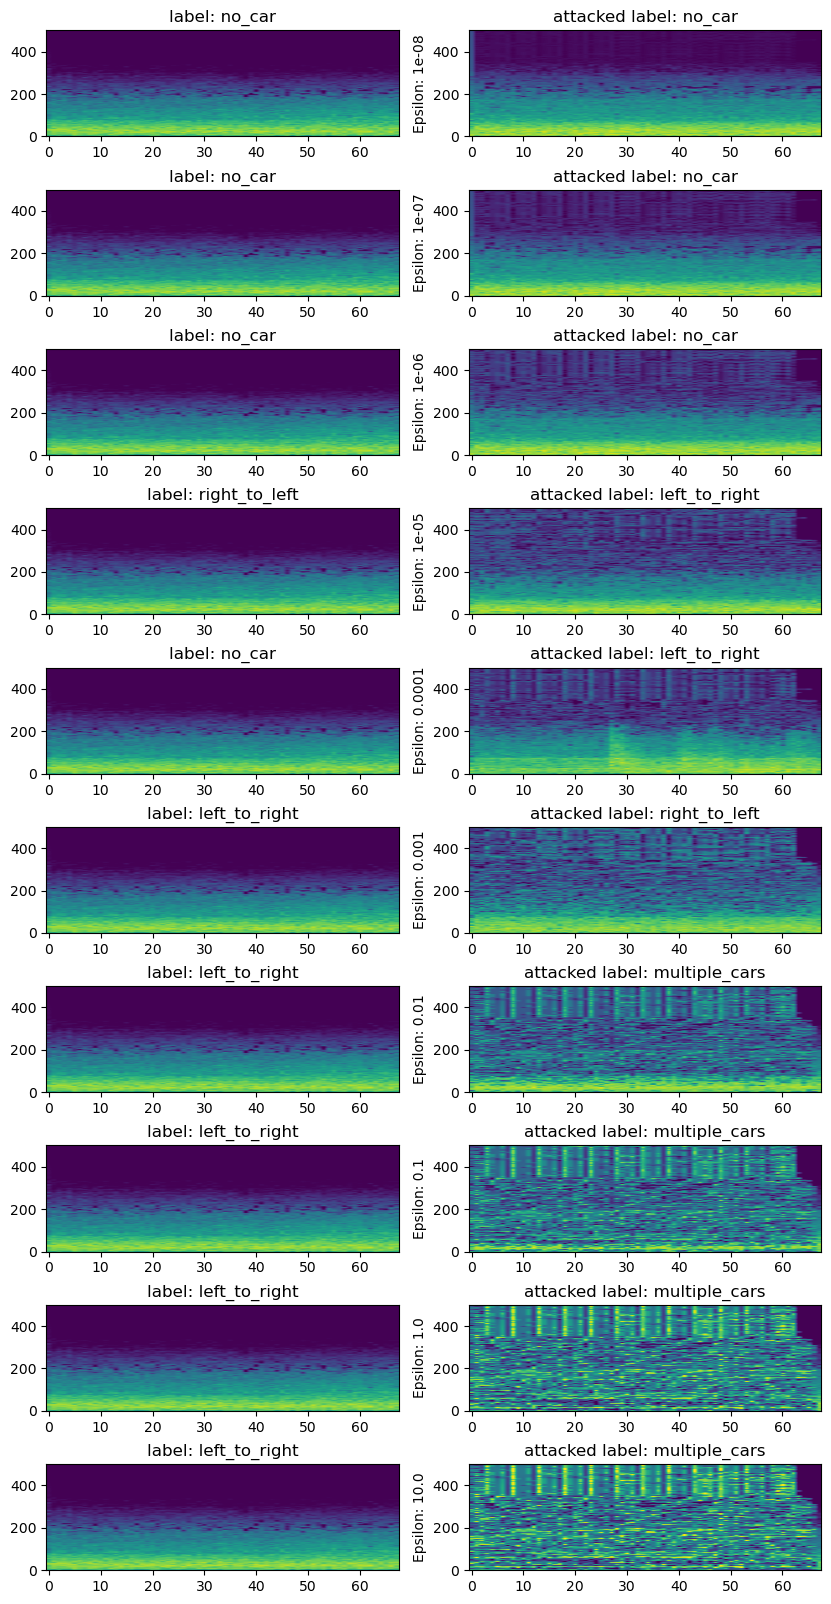
\includegraphics[width=0.8\textwidth]{images/adversarial_attack_results.png}
    \caption{Adversarial attack results}
    \label{fig:adversarial_attack_results}
\end{figure}

This allows us to see that our attack works only when the spectrogram is heavily modified. After reconstructing the audio from the spectrogram, we can hear that the audio is not understandable anymore. It's mainly noise This attack is not useful for our case because we need an audio that will produce the exact spectrogram we modified with the attack.

\subsection{Adversarial Attack mitigation}

We can conclude that a CNN that classifies sounds is safer by design than one that classifies images when attacked with the FGSM. The loss of information during the griffin-lim and the fourier transform makes the model more robust to adversarial attacks. 

Even if we managed to attack with a small $epsilon$, the attack would need to play the sound through a speaker. The speaker would not be able to reproduce every small noise that we added to the spectrogram. So the attack would not work in real life without having a considerably different sound.
By referring to the objective \ref{intro:objective5}, we can conclude that we have partially fulfilled it. We have shown that an adversarial attack is possible but useless in a real-life case. We must find an attack that works differently to fulfill this objective completely.